% This LaTeX was auto-generated from MATLAB code.
% To make changes, update the MATLAB code and export to LaTeX again.

\documentclass{article}

\usepackage[utf8]{inputenc}
\usepackage[T1]{fontenc}
\usepackage{lmodern}
\usepackage{graphicx}
\usepackage{color}
\usepackage{hyperref}
\usepackage{amsmath}
\usepackage{amsfonts}
\usepackage{epstopdf}
\usepackage[table]{xcolor}
\usepackage{matlab}
\usepackage[paperheight=795pt,paperwidth=614pt,top=72pt,bottom=72pt,right=72pt,left=72pt,heightrounded]{geometry}

\sloppy
\epstopdfsetup{outdir=./}
\graphicspath{ {./exam_1_media/} }

\begin{document}

\matlabtitle{Exam 1}

\matlabheadingthree{AME 5763}

\matlabheading{Blake Johnson}


\vspace{1em}

\vspace{1em}
\matlabheading{Problem 1:}


\vspace{1em}
\begin{par}
\begin{flushleft}
Consider the problem of finding the solution of the equation:
\end{flushleft}
\end{par}

\begin{par}
$$\frac{d^2 u}{dx^2 }+u+x=0,~~0<x<1,~~u(0)=u(1)=0$$
\end{par}


\vspace{1em}
\begin{enumerate}
\setlength{\itemsep}{-1ex}
   \item{\begin{flushleft} (25 points)** Develop the weak form. \end{flushleft}}
   \item{\begin{flushleft} (25 points)** Assume trial $u(x)\;\textrm{and}\;\textrm{weight}\;w(x)$ functions with the following form: \end{flushleft}}
\end{enumerate}

\begin{par}
$$u(x)=x(1-x)(\alpha_1 +\alpha_2 x+\cdots +\alpha_N x^{N-1} ),$$
\end{par}


\vspace{1em}
\begin{par}
$$w(x)=x(1-x)(\beta_1 +\beta_2 x+\cdots +\beta_N x^{N-1} ),$$
\end{par}


\vspace{1em}
\begin{par}
\begin{flushleft}
and obtain (but don’t solve) the equations to determine the unknown coefficients $\alpha_i$.
\end{flushleft}
\end{par}


\vspace{1em}
\begin{par}
\begin{flushleft}
 Problem 1 Part 1:
\end{flushleft}
\end{par}

\begin{par}
\begin{flushleft}
The governing diffeential equation is given to us as:
\end{flushleft}
\end{par}

\begin{par}
$$\frac{d^2 u}{dx^2 }+u+x=0$$
\end{par}

\begin{par}
\begin{flushleft}
and the displacement at $x=0$ is the same at $x=1$ which is zero.
\end{flushleft}
\end{par}

\begin{par}
\begin{flushleft}
To find the weak equation, multiply the governing equation by an arbitrary weight function $w(x)$:
\end{flushleft}
\end{par}

\begin{par}
$$w(x)\left\lbrack \frac{d^2 u}{dx^2 }+u+x\right\rbrack =0$$
\end{par}


\vspace{1em}
\begin{par}
$$w(x)\frac{d^2 u}{dx^2 }+w(x)u+w(x)x=0$$
\end{par}


\vspace{1em}
\begin{par}
\begin{flushleft}
now to find the weak form take the integral over the given length $0<x<1$
\end{flushleft}
\end{par}


\vspace{1em}
\begin{par}
$$\int_0^1 \left(w(x)\frac{d^2 u}{dx^2 }+w(x)u+w(x)x\right)dx$$
\end{par}

\begin{par}
$$\int_0^1 w(x)\frac{d^2 u}{dx^2 }dx+\int_0^1 w(x)udx+\int_0^1 w(x)xdx=0$$
\end{par}


\vspace{1em}
\begin{par}
\begin{flushleft}
I used integration by parts for the first term:
\end{flushleft}
\end{par}

\begin{par}
$$\int_0^1 \frac{d^2 u}{dx^2 }dx$$
\end{par}

\begin{par}
$$\begin{array}{l}
u=w(x)\\
du=\frac{dw}{dx}\\
v=\frac{du}{dx}\\
dv=\frac{d^2 u}{dx^2 }
\end{array}$$
\end{par}

\begin{par}
\begin{flushleft}
Integration by parts: $uv-\int vdu$
\end{flushleft}
\end{par}

\begin{par}
$$\int_0^1 w(x)\frac{d^2 u}{dx^2 }dx={\left\lbrack w(x)\frac{du}{dx}\right\rbrack }_0^1 -\int_0^1 \frac{du}{dx}\frac{dw}{dx}dx$$
\end{par}

\begin{par}
\begin{flushleft}
$u(0)=u(1)=0$ is the boundary conditions for the problem. So whatever function $u(x)$ is, it must satisfy these conditions. 
\end{flushleft}
\end{par}

\begin{par}
\begin{flushleft}
Additionally the weight function vanishes at the boundary conditions. So $w(0)=0\;\textrm{and}\;w(1)=0$
\end{flushleft}
\end{par}

\begin{par}
$$\left(w(1)\frac{du}{dx}-w(0)\frac{du}{dx}\right)=0$$
\end{par}

\begin{par}
$$\int_0^1 \frac{d^2 u}{dx^2 }dx=0-\int_0^1 \frac{du}{dx}\frac{dw}{dx}dx$$
\end{par}

\begin{par}
\begin{flushleft}
Now the full integral for the weak form is:
\end{flushleft}
\end{par}

\begin{par}
$$\int_0^1 w(x)\frac{d^2 u}{dx^2 }dx+\int_0^1 w(x)udx+\int_0^1 w(x)xdx=0=-\int_0^1 \frac{du}{dx}\frac{dw}{dx}dx+\int_0^1 w(x)udx+\int_0^1 w(x)xdx=0$$
\end{par}

\begin{par}
\begin{flushleft}
Since the problem does not provide test functions, this is about as simplified as it can get. So the weak form is:
\end{flushleft}
\end{par}

\begin{par}
$$\int_0^1 w(x)udx+\int_0^1 w(x)xdx=\int_0^1 \frac{du}{dx}\frac{dw}{dx}dx$$
\end{par}

\begin{par}
\begin{flushleft}
Part 2:
\end{flushleft}
\end{par}

\begin{par}
\begin{flushleft}
Here I want to try to input the u(x) and w(x) given in the assignment into the weak form to solve.
\end{flushleft}
\end{par}

\begin{par}
\begin{flushleft}
if we consider the trial functions:
\end{flushleft}
\end{par}

\begin{par}
$$\begin{array}{l}
u(x)=x(1-x)(\alpha_1 +\alpha_2 x+...+\alpha_N x^{N-1} )\\
w(x)=x(1-x)(\beta_1 +\beta_2 x+...+\beta_N x^{N-1} )\\
\frac{du}{dx}=(1-2x)((n-1)\alpha_N x^{N-2} +...+\alpha_2 )\\
\frac{dw}{dx}=(1-2x)((n-1)\beta_N x^{N-2} +...+\beta_2 )
\end{array}$$
\end{par}

\begin{par}
\begin{flushleft}
and then we have:
\end{flushleft}
\end{par}

\begin{par}
$$\begin{array}{l}
\int_0^1 w(x)udx+\int_0^1 w(x)xdx=\int_0^1 \frac{du}{dx}\frac{dw}{dx}dx=\\
\int_0^1 [x(1-x)(\beta_1 +\beta_2 x+...+\beta_N x^{N-1} )][x(1-x)(\alpha_1 +\alpha_2 x+...+\alpha_N x^{N-1} )]dx+\int_0^1 [x(1-x)(\beta_1 +\beta_2 x+...+\beta_N x^{N-1} )]dx=\\
\int_0^1 (1-2x)^2 ((N-1)\alpha_n x^{n-2} +...+\alpha )\beta_n x^{n-2} +...+\beta )dx
\end{array}$$
\end{par}

\begin{par}
\begin{flushleft}
Here I could solve for $\alpha_i$if i knew the value. The math is a little messy for me to try and go much further. We know that the integration is going to be of some unknown exponent, so the integration will take on some form of $\int x^{exp} dx=\frac{1}{exp+1}$ but that is about all I know to do here without an exact value.
\end{flushleft}
\end{par}

\begin{par}
\begin{flushleft}
Additionally I considered the idea that we could set the problem up this way:
\end{flushleft}
\end{par}

\begin{par}
$$\begin{array}{l}
\frac{d^2 u}{dx^2 }+u+x=0\\
\frac{d^2 u}{dx^2 }=-u-x\\
\int \frac{d^2 u}{dx^2 }dx=\int -udx-\int xdx\\

\end{array}$$
\end{par}

\begin{par}
\begin{flushleft}
Then we could integrate for and potentially solve for an $\alpha_{specific}$ which would let us determine any $a_i$ from that point. This is what I did for homework 1 question 3.14 when I solved for $\alpha_3$ but I dont think that is quite a feasible as:	
\end{flushleft}
\end{par}

\begin{par}
$$\begin{array}{l}
\int_0^1 [x(1-x)(\beta_1 +\beta_2 x+...+\beta_N x^{N-1} )][x(1-x)(\alpha_1 +\alpha_2 x+...+\alpha_N x^{N-1} )]dx+\int_0^1 [x(1-x)(\beta_1 +\beta_2 x+...+\beta_N x^{N-1} )]dx=\\
\int_0^1 (1-2x)^2 ((N-1)\alpha_n x^{n-2} +...+\alpha )\beta_n x^{n-2} +...+\beta )dx
\end{array}$$			
\end{par}

\matlabheading{Problem 2:					}

\begin{par}
\begin{flushleft}
Verify that the shape functions of two-, three- and four-node elements derived in this chapter satisfy the following conditions: 			
\end{flushleft}
\end{par}

\begin{par}
$$\sum_{I=1}^{n_{en} } N_I^e (x)=1$$
\end{par}

\begin{par}
\begin{flushleft}
Explain why the above condition always has to be satisfied. 
\end{flushleft}
\end{par}

\begin{par}
\begin{flushleft}
I did this problem by hand for the two and three nodes the fourth node was messy, so I decided to use MATLAB to show my results. I used the direct construction of shape functions in one dimension from section 4.3 to solve these probelms. 
\end{flushleft}
\end{par}

\begin{par}
\begin{flushleft}
Two Node:
\end{flushleft}
\end{par}

\begin{par}
$$N_1 (x)=\frac{(x-x_2 )}{(x_1 -x_2 )}\textrm{and}\;N_2 (x)=\frac{(x-x_1 )}{(x_2 -x_1 )}$$
\end{par}

\begin{par}
$$\sum_{I=1}^2 N_I (x)=\frac{(x-x_2 )}{(x_1 -x_2 )}+\frac{(x-x_1 )}{(x_2 -x_1 )}=1$$
\end{par}

\begin{par}
$$\frac{(x-x_2 )}{(x_1 -x_2 )}-\frac{(x-x_1 )}{(x_1 -x_2 )}=1$$
\end{par}

\begin{par}
$$\frac{(x-x_2 )-(x-x_1 )}{(x_1 -x_2 )}=1$$
\end{par}

\begin{par}
$$\frac{x-x_2 -x+x_1 }{(x_1 -x_2 )}=1$$
\end{par}

\begin{par}
$$\frac{(x_1 -x_2 )}{(x_1 -x_2 )}=1$$
\end{par}

\begin{par}
$$1=1$$
\end{par}

\begin{par}
\begin{flushleft}
Three Node:
\end{flushleft}
\end{par}

\begin{par}
$$N_1 (x)=\frac{(x-x_2 )(x-x_3 )}{(x_1 -x_2 )(x_1 -x_3 )}\;\textrm{;}\;N_2 (x)=\frac{(x-x_1 )(x-x_3 )}{(x_2 -x_1 )(x_2 -x_3 )}\;\textrm{;}\;N_3 (x)=\frac{(x-x_1 )(x-x_2 )}{(x_3 -x_1 )(x_3 -x_2 )}$$
\end{par}

\begin{par}
\begin{flushleft}
Moving forward let: $x_1 =A\;\textrm{,}\;x_2 =B\;\textrm{,}\;\textrm{and}x_3 =C$		
\end{flushleft}
\end{par}

\begin{par}
$$N_1 (x)=\frac{(x-B)(x-C)}{(A-B)(A-C)}\;\textrm{;}\;N_2 (x)=\frac{(x-A)(x-C)}{(B-A)(B-C)}\;\textrm{;}\;N_3 (x)=\frac{(x-A)(x-B)}{(C-A)(C-B)}$$
\end{par}

\begin{par}
\begin{center}
		
\end{center}
\end{par}

\begin{par}
$$\frac{(x-B)(x-C)}{(A-B)(A-C)}+\frac{(x-A)(x-C)}{(B-A)(B-C)}+\frac{(x-A)(x-B)}{(C-A)(C-B)}=1$$
\end{par}


\vspace{1em}
\begin{par}
$$\frac{(x-B)(x-C)(B-C)}{(A-B)(A-C)(B-C)}-\frac{(x-A)(x-C)(A-C)}{(A-B)(B-C)(A-C)}+\frac{(x-A)(x-B)(A-B)}{(A-C)(B-C)(A-B)}=1$$
\end{par}


\vspace{1em}
\begin{par}
$$\frac{[(x-B)(x-C)(B-C)]-[(A-B)(A-C)(B-C)]+[(x-A)(x-B)(A-B)]}{(A-C)(B-C)(A-B)}=1$$
\end{par}

\begin{par}
\begin{flushleft}
I did a lot of expanding out on paper to get the following:
\end{flushleft}
\end{par}


\vspace{1em}
\begin{par}
$$\frac{-A^2 C-AC^2 +B^2 C-BC^2 +A^2 B-AB^2 }{(A-C)(B-C)(A-B)}=1$$
\end{par}


\vspace{1em}
\begin{par}
\begin{flushleft}
I then expanded the denomenator to get:
\end{flushleft}
\end{par}


\vspace{1em}
\begin{par}
$$\frac{-A^2 C-AC^2 +B^2 C-BC^2 +A^2 B-AB^2 }{-A^2 C-AC^2 +B^2 C-BC^2 +A^2 B-AB^2 }=1$$
\end{par}


\vspace{1em}
\begin{par}
$$1=1$$
\end{par}

\begin{par}
\begin{flushleft}
Four Node:
\end{flushleft}
\end{par}

\begin{par}
\begin{flushleft}
For the four nodes I found an interesting pattern when I tried to manually force the values like I did above. I began the same way as above:
\end{flushleft}
\end{par}

\begin{par}
$$\begin{array}{l}
N_1 (x)=\frac{(x-x_2 )(x-x_3 (x-x_4 )}{(x_1 -x_2 )(x_1 -x_3 )(x_1 -x_4 )}\;\textrm{;}\;N_2 (x)=\frac{(x-x_1 )(x-x_3 )(x-x_4 )}{(x_2 -x_1 )(x_2 -x_3 )(x_2 -x_4 )}\;\textrm{;}\;\\
N_3 (x)=\frac{(x-x_1 )(x-x_2 )(x-x_4 )}{(x_3 -x_1 )(x_3 -x_2 )(x_3 -x_4 }\;\textrm{and}\;N_4 (x)=\frac{(x-x_1 )(x-x_2 )(x-x_3 )}{(x_4 -x_1 )(x_4 -x_2 )(x_4 -x_3 }
\end{array}$$
\end{par}

\begin{par}
\begin{flushleft}
Again I set the values $x_1 =A\;\textrm{,}\;x_2 =B\;\textrm{,}\;x_3 =C\;\textrm{,}\;\textrm{and}x_4 =D$
\end{flushleft}
\end{par}

\begin{par}
\begin{flushleft}
But this time I noticed that in order for the values to equal 1, the numerator must match the denominator. And there are no x values in the denominator, which means that the coefficients must equal zero in the numerator. So I expanded the equations to get:
\end{flushleft}
\end{par}

\begin{par}
$$\begin{array}{l}
N_1 +N_2 +N_3 +N_4 =\\
\frac{(x-C)(x-D)(C-D)[(x-B)(B-C)(B-D)-(X-A)(A-C)(A-D)]+(x-A)(x-B)(A-B)[(x-D)(A-D)(B-D)-(x-C)(A-C)(B-C)]}{(A-B)(A-C)(A-D)(B-C)(B-D)}
\end{array}$$
\end{par}

\begin{par}
\begin{flushleft}
Since I am interested in the coefficients at the variables I set the denominator aside and expanded the numerator. Then I moved all the factors that contained a variable to the front and go the following:
\end{flushleft}
\end{par}

\begin{par}
$$\begin{array}{l}
+(x-B)(x-C)(x-D)(B-C)(B-D)(C-D)\\
-[(x-A)(x-C)(x-D)(A-C)(A-D)(C-D)]\\
+[(x-A)(x-B)(x-D)(A-B)(A-D)(B-D)]\\
-[(x-A)(x-B)(x-C)(A-B)(A-C)(B-C)]
\end{array}$$
\end{par}

\begin{par}
\begin{flushleft}
So my thinking is that if the numerator and denominator are equal then the coefficients infront of each variable must be equal to zero. If i expand out the first three factor, the first term will be $x^3$, meaning that the last three factors in each section must be the coefficient to $x^3$.
\end{flushleft}
\end{par}

\begin{par}
\begin{flushleft}
In other words the first term will expand to:
\end{flushleft}
\end{par}

\begin{par}
$$[(B-C)(B-D)(C-D)]x^3 -[(A-C)(A-D)(C-D)]x^3 +[(A-B)(A-D)(B-D)]x^3 -[(A-B)(A-C)(B-C)]x^3$$
\end{par}

\begin{par}
\begin{flushleft}
So, I expand that out and get the following four equations (I know they technically are not equations, but I feel like that is the best term I have for them right now):
\end{flushleft}
\end{par}

\begin{par}
$$\begin{array}{l}
\;\textrm{1.)}\;+B^2 C-BC^2 +C^2 D-B^2 D+BD^2 +CD^2 \\
\;\textrm{2.)}\;-A^2 C+AC^2 -C^2 D+A^2 D_A D^2 +CD^2 \\
\;\textrm{3.)}\;+A^2 B-AB^2 +B^2 D-A^2 D+AD^2 -BD^2 \\
\;\textrm{4.)}\;-A^2 B+AB^2 -B^2 C+A^2 C-AC^2 +BC^2 
\end{array}$$
\end{par}

\begin{par}
\begin{flushleft}
Now when we add these together they will cancel to zero, showing that the coefficient of $x^3$ is zero.
\end{flushleft}
\end{par}

\begin{par}
\begin{flushleft}
Now for the $x^2$section we get some interesting results. Now the $x^2$ term also includes the numbers in the factors, that were not considered in the $x^3$ coefficient. But, notice that all we are doing is increasing each exponent by a value of 1 and flipping the sign. So we can say without really doing any math that these two must be zero. Since they all we are doing is changing the values of each equation proportionally.  
\end{flushleft}
\end{par}

\begin{par}
$$\begin{array}{l}
\;\textrm{1.)}\;+B^3 C-B^2 C^2 +bC^2 D-B^3 D+B^2 D^2 +BCD^2 +B^2 C^2 -BC^3 +C^3 D-B^2 CD+BCD^2 +C^2 D^2 +B^2 CD-BC^2 D+C^2 D^2 -B^2 D^2 +BD^3 +CD^3 \\
\;\textrm{2.)}\;-A^3 C+A^2 C^2 -AC^2 D+A^3 D-A^2 D^2 +ACD^2 -A^2 C^2 +AC^3 -C^3 D+A^2 CD-ACD^2 +C^2 D^2 -A^2 CD+AC^2 D-C^2 D^2 +A^2 D^2 -AD^3 +CD^3 \\
\;\textrm{3.)}\;+A^3 B-A^2 B^2 +AB^2 D-A^3 D+A^2 D^2 -ABD^2 +A^2 B^2 -AB^3 +B^3 D-A^2 BD+ABD^2 -B^2 D^2 +A^2 BD-AB^2 D+B^2 D^2 -A^2 D^2 +AD^3 -BD^3 \\
\;\textrm{4.)}\;-A^3 B+A^2 B^2 -AB^2 C+A^3 C-A^2 C^2 +ABC^2 -A^2 B^2 +AB^3 -B^3 C+A^2 BC-ABC^2 +B^2 C^2 -A^2 BC+AB^2 C-B^2 C^2 +A^2 C^2 -AC^3 +BC^3 
\end{array}$$
\end{par}

\begin{par}
\begin{flushleft}
And again they will cancel.
\end{flushleft}
\end{par}

\begin{par}
\begin{flushleft}
For the variable x we have a similar pattern. I noticed that the BC values in equations 1 canceled with equation 4. So when we multiply the coefficients of the x term in equations 1 and 4, nothing will change. The CD terms cancel in equations one and two which happen to also be the two equations that multiply their x coefficients by CD. This pattern continues for all of the multiples for the x variable. Again this means that we are proportionally increasing the coefficients proportionally and they will cancel.
\end{flushleft}
\end{par}

\begin{par}
\begin{flushleft}
Now we just focus on the constant terms at the end of the equations. When the constant terms are multiplied to the remaining values we can no longer just cancel them:
\end{flushleft}
\end{par}

\begin{par}
$$\begin{array}{l}
\;\textrm{1.)}\;+B^3 C^2 D-B^2 C^3 D+BC^3 D^2 -B^3 CD^2 +B^2 CD^3 +BC^2 D^3 \\
\;\textrm{2.)}\;-A^3 C^2 D+A^2 C^3 D-AC^3 D^2 +A^3 CD^2 -A^2 CD^3 +AC^2 D^3 \\
\;\textrm{3.)}\;+A^3 B^2 D-A^2 B^3 D+AB^3 D^2 -A^3 BD^2 +A^2 BD^3 -AB^2 D^3 \\
\;\textrm{4.)}\;-A^3 B^2 C+A^2 B^3 C-AB^3 C^2 +A^3 BC^2 -A^2 BC^3 +AB^2 C^3 
\end{array}$$
\end{par}

\begin{par}
\begin{flushleft}
This reduces down and our denominator expands to:
\end{flushleft}
\end{par}

\begin{par}
$$\frac{D^2 C^3 -D^3 C^2 +A^2 CB^2 -DA^2 B^2 +D^2 A^2 B-A^2 C^2 B+DA^2 C^2 -D^2 A^2 C+AD^2 B^2 -AD^3 B+AD^3 C-AC^2 B^2 +AC^3 B-DAC^3 +DC^2 B^2 -D^2 CB^2 +D^3 CB-DC^3 B-AD^2 CB+DAC^2 B}{D^2 C^3 -D^3 C^2 +A^2 CB^2 -DA^2 B^2 +D^2 A^2 B-A^2 C^2 B+DA^2 C^2 -D^2 A^2 C+AD^2 B^2 -AD^3 B+AD^3 C-AC^2 B^2 +AC^3 B-DAC^3 +DC^2 B^2 -D^2 CB^2 +D^3 CB-DC^3 B-AD^2 CB+DAC^2 B}=1$$
\end{par}

\begin{par}
\begin{flushleft}
The shape functions provide the displacement (or other field variable) of the element at that specific node. So at node 1 $N_1 =1$ but $N_2 =0$, $N_3 =0$ and so on. Similarly at node 2 $N_2 =1$, but  $N_1 =0$ and $N_3 =0$. This ensures that there is a smooth continuous function in our Finite Element which is crucial to solving the equations. This is why this is so important.
\end{flushleft}
\end{par}


\vspace{1em}
\matlabheading{Problem 3:}

\begin{par}
\begin{flushleft}
Repeat book problem 4.4d using a 3 noded element where the trial and weight function approximations are given by the incomplete polynomial (but with a linear complete approximation): $\theta_e =\alpha_e^0 +\alpha_e^1 x+\alpha_e^2 x^4$ Compare the results to the linear approximation.
\end{flushleft}
\end{par}


\vspace{1em}
\begin{par}
\begin{flushleft}
The following code is a modified form of what I used for homework 4.4.
\end{flushleft}
\end{par}

\begin{matlabcode}
% Define the exact solution u(x) = x^3 as an anonymous function
exact_solution = @(x) x.^3;

% Define the Gauss quadrature points and weights for a 3-point rule
gauss_points = [-sqrt(3/5), 0, sqrt(3/5)];  % Gauss points in [-1, 1]
gauss_weights = [5/9, 8/9, 5/9];  % Weights for 3-point quadrature

% Initialize an array to store the L2 norm error for 2, 4, and 8 elements
error_L2 = zeros(3, 1);  % To store errors for each mesh size

% Define the mesh sizes
mesh_sizes = [2, 4, 8];
L = 1;  % Length of the domain

% Loop over each mesh size
for mesh_index = 1:length(mesh_sizes)
    num_elements = mesh_sizes(mesh_index);  % Get the number of elements
    element_length = L / num_elements;  % Compute the length of each element
    error_sum = 0;  % Initialize the error sum for this mesh size

    % Loop over each element
    for elem = 1:num_elements
        % Define element boundaries for the three nodes
        x1 = (elem - 1) * element_length;  % Left node of element
        x2 = x1 + element_length / 2;      % Middle node of element
        x3 = elem * element_length;        % Right node of element

        % Quadratic shape functions for the element
        u_h = @(x) ((x - x2)*(x - x3))/((x1 - x2)*(x1 - x3)) * exact_solution(x1) + ...
                   ((x - x1)*(x - x3))/((x2 - x1)*(x2 - x3)) * exact_solution(x2) + ...
                   ((x - x1)*(x - x2))/((x3 - x1)*(x3 - x2)) * exact_solution(x3);

        % Compute the squared error for each Gauss point
        for i = 1:length(gauss_points)
            % Map Gauss point to the actual element
            xi = ((x3 - x1) / 2) * gauss_points(i) + (x3 + x1) / 2;

            % Compute the error at the Gauss point
            error_at_gauss_point = (u_h(xi) - exact_solution(xi))^2;

            % Sum the contribution of this Gauss point
            error_sum = error_sum + gauss_weights(i) * error_at_gauss_point * (x3 - x1) / 2;
        end
    end

    % Store the L2 norm error for this mesh size
    error_L2(mesh_index) = sqrt(error_sum);
end

% Plot the error vs element size (log-log plot)
element_sizes = 1 ./ mesh_sizes;  % Element size = 1 / number of elements
figure;
loglog(element_sizes, error_L2, '-o', 'LineWidth', 2);
xlabel('Element Size (h)');
ylabel('L2 Norm of Error');
title('L2 Norm Error vs Element Size');
grid on;
\end{matlabcode}
\begin{center}
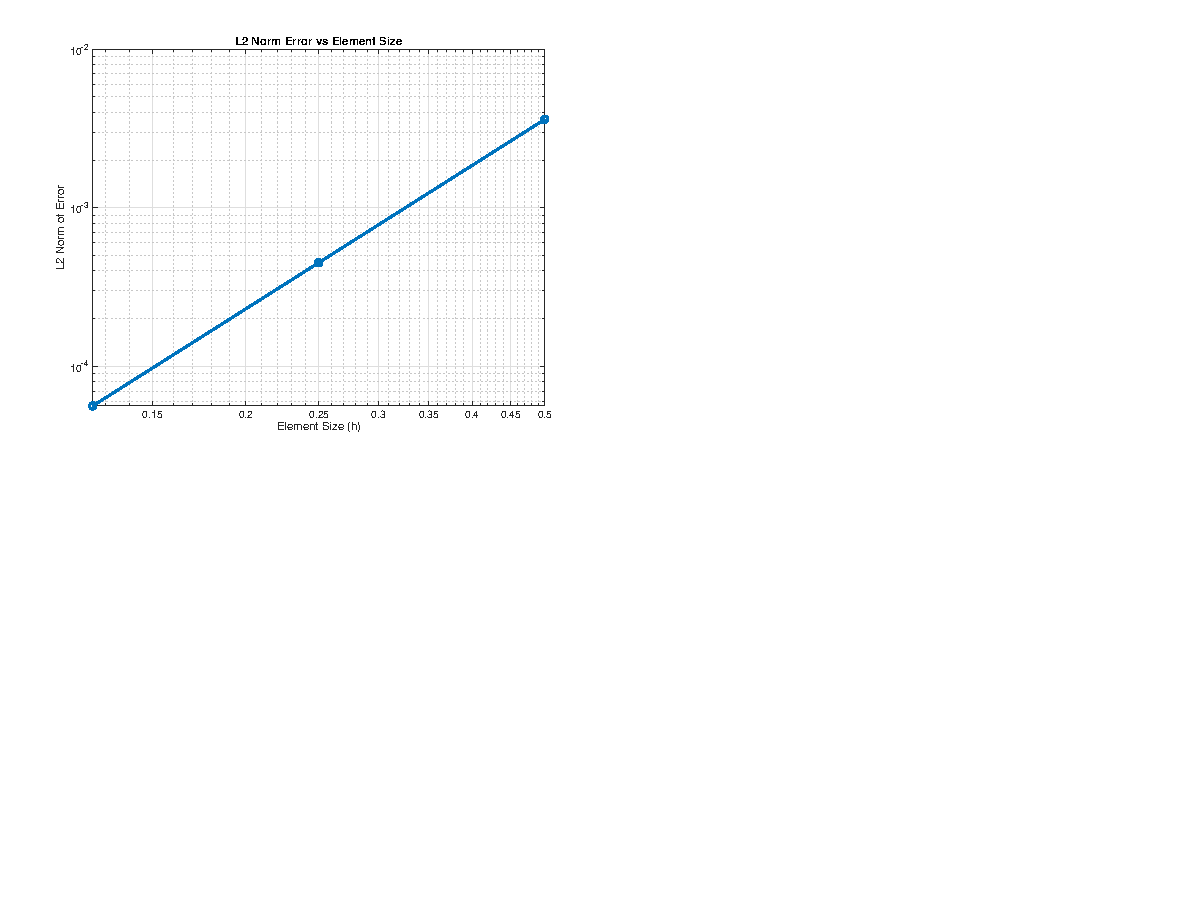
\includegraphics[width=\maxwidth{56.196688409433015em}]{figure_0.eps}
\end{center}
\begin{matlabcode}

% Optionally, compute the slope of the log-log plot (convergence rate)
p = polyfit(log(element_sizes), log(error_L2), 1);
fprintf('Slope of the log-log plot (rate of convergence): %.2f\n', p(1));
\end{matlabcode}
\begin{matlaboutput}
Slope of the log-log plot (rate of convergence): 3.00
\end{matlaboutput}

\begin{par}
\begin{flushleft}
I also tried to use your code and came up with the following:
\end{flushleft}
\end{par}

\begin{matlabcode}

%%%%%%%%%%%%%%%%%%%%%%%%%%%%%%%%%%%%%%%%%%%%%%%%%%%%%%%%%%%%%%%%%%%%%%%%%%%%%%%%%%%
% User input
%%%%%%%%%%%%%%%%%%%%%%%%%%%%%%%%%%%%%%%%%%%%%%%%%%%%%%%%%%%%%%%%%%%%%%%%%%%%%%%%%%%

%Element type
% etype=1: linear 2 node element
% etype=2: quadratic 3 node element
etype = 2;  % Change this to 1 for linear elements, 2 for quadratic elements

% Number of elements
Nelem = 8;

% Number of points to plot within each element
Npp = 10;

%%%%%%%%%%%%%%%%%%%%%%%%%%%%%%%%%%%%%%%%%%%%%%%%%%%%%%%%%%%%%%%%%%%%%%%%%%%%%%%%%%
% End User input
%%%%%%%%%%%%%%%%%%%%%%%%%%%%%%%%%%%%%%%%%%%%%%%%%%%%%%%%%%%%%%%%%%%%%%%%%%%%%%%%%%

% Domain length
L = 1.0;

% 1 dof per node
Ndof = 1;

% Nnodes: number of nodes per element
% Nnodes_g: number of global nodes
if etype == 1
    Nnodes = 2;
    Nnodes_g = Nelem + 1;
else
    Nnodes = 3;  % 3-node quadratic element
    Nnodes_g = 2 * Nelem + 1;  % Global nodes for quadratic elements
end

% Element length in 1D; constant throughout here
dx = L / Nelem;

% Spacing between plotting points (Gauss quadrature domain [-1,1])
dxi_plot = 2.0 / (Npp - 1);

% Initialize arrays for node coordinates
xyz = zeros(Nnodes_g, 3);
for i = 1:Nnodes_g
    xyz(i,1) = (i-1)*(dx/(Nnodes-1));
end

% Define element node to global node mapping (adjusted for 3-node element)
elem_map = zeros(Nelem, Nnodes);
for i = 1:Nelem
    for j = 1:Nnodes
        elem_map(i,j) = (i-1)*2 + j;  % Adjusted for quadratic elements
    end
end

% Define total number of global dof
Ndof_tot = Nnodes_g * Ndof;

%%%%%%%%%%%%%%%%%%%%%%%%%%%%%%%%%%%%%%%%%%%%%%%%%%
% Initialize all arrays with zeros
%%%%%%%%%%%%%%%%%%%%%%%%%%%%%%%%%%%%%%%%%%%%%%%%%%
D = zeros(Ndof_tot,1);
ue = zeros(Nelem,Npp);
uexact = zeros(Nelem,Npp);
ee = zeros(Nelem,Npp);
eexact = zeros(Nelem,Npp);
xe = zeros(Nelem,Npp);
Delem = zeros(Nnodes,1);
xelem = zeros(Nnodes,1);
xi = zeros(4,1);

f1 = figure;
f2 = figure;
err2 = 0.0;

% Assign values to D based on exact solution u_I=x_I^3
for i = 1:Ndof_tot
    D(i) = xyz(i,1)^3;
end

% Loop over elements
for i = 1:Nelem

    % Assign nodal displacements and positions using elem_map
    for j = 1:Nnodes
        Delem(j,1) = D(elem_map(i,j));
        xelem(j,1) = xyz(elem_map(i,j));
    end

    % Loop over element plotting points
    for j = 1:Npp

        % Plotting point (in -1 to 1 domain)
        xi(1) = -1.0 + (j-1) * dxi_plot;

        % Compute shape function and B matrix
        if etype == 1
            xe(i,j) = xelem(1,1) * 0.5 * (1.0 - xi(1)) + xelem(2,1) * 0.5 * (1.0 + xi(1));
            [N, B] = shape1d_lin(xe(i,j), xelem);
        elseif etype == 2
            % Correct quadratic mapping
            xe(i,j) = xelem(1,1) * (xi(1) * (xi(1) - 1)) / 2 + ...
                      xelem(2,1) * (1 - xi(1)^2) + ...
                      xelem(3,1) * (xi(1) * (xi(1) + 1)) / 2;
            [N, B] = shape1d_quad(xe(i,j), xelem);  % Use quadratic shape function
        end

        % Displacement and strain at xe(j)
        ue(i,j) = N * Delem;
        uexact(i,j) = xe(i,j)^3;
        ee(i,j) = B * Delem;
        eexact(i,j) = 3.0 * xe(i,j)^2;
    end

    %%%%%%%%%%%%%%%%%%%%%%%%%%%%%%%%%%%%%%%%%%%%%%
    % Error calculation (Parts d and e)
    %%%%%%%%%%%%%%%%%%%%%%%%%%%%%%%%%%%%%%%%%%%%%%

    % Use four-point Gauss quadrature for exact solution (cubic)
    w = [0.3478548451, 0.3478548451, 0.6521451549, 0.6521451549];
    xi = [0.8611363116, -0.8611363116, 0.3399810436, -0.3399810436];

    % Element length
    if etype == 1
        le = xelem(2) - xelem(1);
    else
        le = xelem(3) - xelem(1);
    end

    % Jacobian for transformation between x and xi
    Jac = 0.5 * le;

    % Loop over Gauss quad points
    for j = 1:4
        if etype == 1
            xg = xelem(1,1) * 0.5 * (1.0 - xi(j)) + xelem(2,1) * 0.5 * (1.0 + xi(j));
            [N, B] = shape1d_lin(xg, xelem);
        elseif etype == 2
            xg = xelem(1,1) * (xi(j) * (xi(j) - 1)) / 2 + ...
                 xelem(2,1) * (1 - xi(j)^2) + ...
                 xelem(3,1) * (xi(j) * (xi(j) + 1)) / 2;
            [N, B] = shape1d_quad(xg, xelem);
        end

        % Approximation and exact solution at Gauss point
        ue_g = N * Delem;
        uexact_g = xg^3;

        % Compute error
        err2 = err2 + (uexact_g - ue_g)^2 * w(j) * Jac;
    end
end

% Plot results (parts a-c)
for i = 1:Nelem
    figure(f1)
    plot(xe(i,:), ue(i,:), '--', xe(i,:), uexact(i,:));
    legend('Element approximation', 'Exact');
    xlabel('x');
    ylabel('Displacement');
    hold on;
    figure(f2);
    plot(xe(i,:), ee(i,:), '--', xe(i,:), eexact(i,:));
    legend('Element approximation', 'Exact');
    xlabel('x');
    ylabel('Strain');
    hold on;
end
\end{matlabcode}
\begin{center}
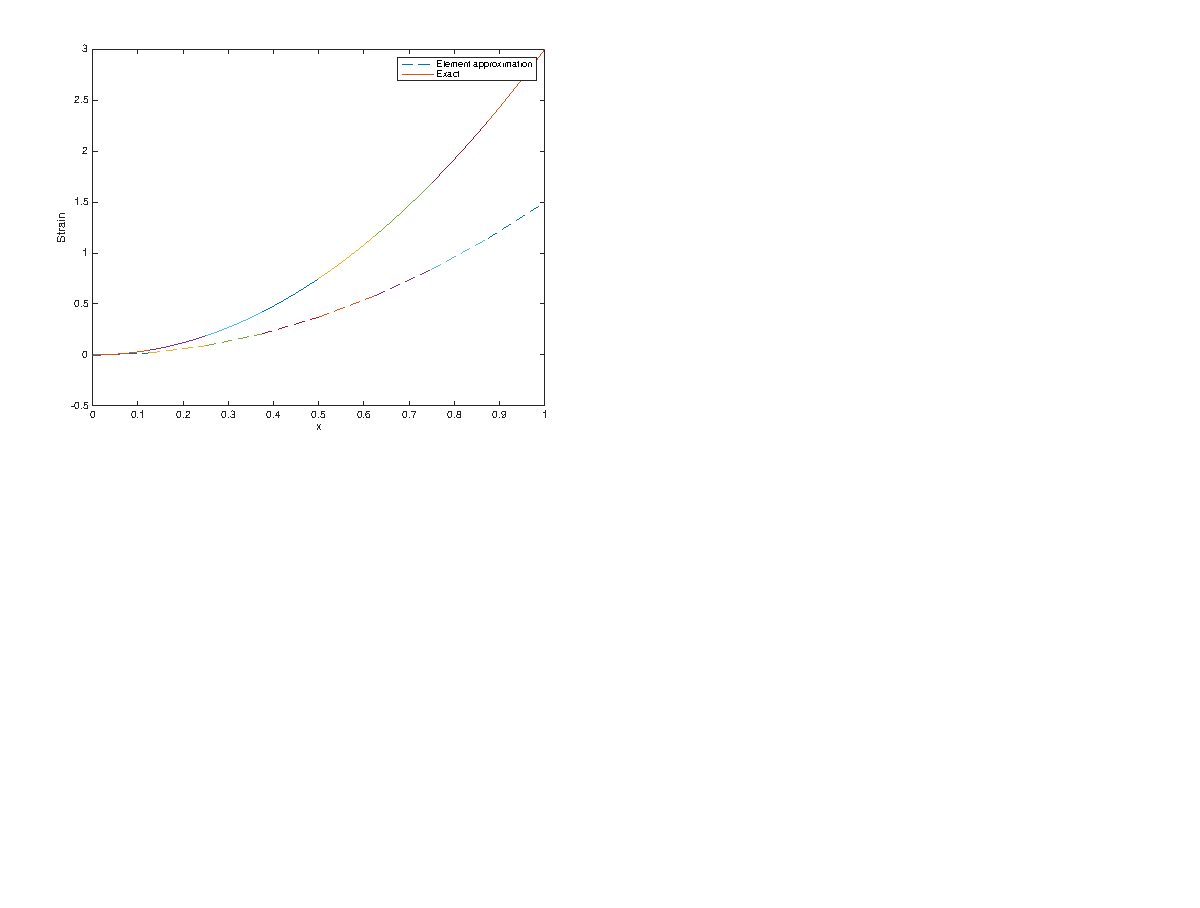
\includegraphics[width=\maxwidth{56.196688409433015em}]{figure_1.eps}
\end{center}
\begin{matlabcode}

%%%%%%%%%%%%%%%%%%%%%%%%%%%%%%%%%%%%%%%%%%%%%%%%%%%%%%%%%%%%%%%%%%%%%%%%%%%%%%%%%%
% Shape Function for 2-Node Linear Element
%%%%%%%%%%%%%%%%%%%%%%%%%%%%%%%%%%%%%%%%%%%%%%%%%%%%%%%%%%%%%%%%%%%%%%%%%%%%%%%%%%
function [N, B] = shape1d_lin(x, xelem)
    le = xelem(2) - xelem(1);  % Element length
    xi = (2*(x - xelem(1)) / le) - 1;  % Parametric coordinate in [-1, 1]

    % Shape functions for 2-node linear element
    N = [(1 - xi) / 2, (1 + xi) / 2];
    
    % Derivative of shape functions (B matrix)
    B = [-1 / le, 1 / le];
end

%%%%%%%%%%%%%%%%%%%%%%%%%%%%%%%%%%%%%%%%%%%%%%%%%%%%%%%%%%%%%%%%%%%%%%%%%%%%%%%%%%
% Shape Function for 3-Node Quadratic Element
%%%%%%%%%%%%%%%%%%%%%%%%%%%%%%%%%%%%%%%%%%%%%%%%%%%%%%%%%%%%%%%%%%%%%%%%%%%%%%%%%%
function [N, B] = shape1d_quad(x, xelem)
    le = xelem(3) - xelem(1);  % Element length
    xi = 2 * (x - xelem(1)) / le - 1;  % Parametric coordinate in [-1, 1]

    % Shape functions for 3-node quadratic element
    N = [(xi*(xi-1))/2, (1-xi^2), (xi*(xi+1))/2];

    % Derivative of shape functions (B matrix)
    B = [(xi - 0.5), -2*xi, (xi + 0.5)] / le;
end


\end{matlabcode}

\begin{par}
\begin{flushleft}
When we compare these to the linear approximations we see that there is a much greater accuracy. As we increase in nodes and as the test functions increase in their orders the accuracy improves drastically. I did try to run some plots to help compare but I was running into some coding problems and was running out of time.
\end{flushleft}
\end{par}

\begin{matlabcode}
%%%%%%%%%%%%%%%%%%%%%%%%%%%%%%%%%%%%%%%%%%%%%%%%%%%%%%%%%%%%%%%%%%%%%%%%%%%%%%%%%%
% Modified Code for a 3-node element with incomplete polynomial approximation
% \sigma^{e} = \alpha_0^{e} + \alpha_1^{e} x + \alpha_2^{e} x^4
%%%%%%%%%%%%%%%%%%%%%%%%%%%%%%%%%%%%%%%%%%%%%%%%%%%%%%%%%%%%%%%%%%%%%%%%%%%%%%%%%%


% Define the exact solution u(x) = x^3 as an anonymous function
exact_solution = @(x) x.^3;

% Define the Gauss quadrature points and weights for a 3-point rule
gauss_points = [-sqrt(3/5), 0, sqrt(3/5)];  % Gauss points in [-1, 1]
gauss_weights = [5/9, 8/9, 5/9];  % Weights for 3-point quadrature

% Initialize an array to store the L2 norm error for 2, 4, and 8 elements
error_L2_incomplete = zeros(3, 1);  % Error for incomplete polynomial
error_L2_linear = zeros(3, 1);  % Error for linear approximation

% Define the mesh sizes
mesh_sizes = [2, 4, 8];
L = 1;  % Length of the domain

% Loop over each mesh size
for mesh_index = 1:length(mesh_sizes)
    num_elements = mesh_sizes(mesh_index);  % Get the number of elements
    element_length = L / num_elements;  % Compute the length of each element
    error_sum_incomplete = 0;  % Initialize error sum for incomplete polynomial
    error_sum_linear = 0;  % Initialize error sum for linear approximation

    % Loop over each element
    for elem = 1:num_elements
        % Define element boundaries and mid-point
        x1 = (elem - 1) * element_length;  % Left node of element
        x3 = elem * element_length;        % Right node of element
        x2 = (x1 + x3) / 2;               % Mid-point of element

        % Finite element approximation using incomplete polynomial (x, x^4)
        N1_incomplete = @(x) (x - x2) * (x - x3) / ((x1 - x2) * (x1 - x3));
        N2_incomplete = @(x) (x - x1) * (x - x3) / ((x2 - x1) * (x2 - x3));
        N3_incomplete = @(x) (x - x1) * (x - x2) / ((x3 - x1) * (x3 - x2));

        u_h_incomplete = @(x) N1_incomplete(x) * exact_solution(x1) + N2_incomplete(x) * exact_solution(x2) + N3_incomplete(x) * exact_solution(x3);

        % Linear approximation for comparison
        u_h_linear = @(x) ((x3 - x) / element_length) * exact_solution(x1) + ((x - x1) / element_length) * exact_solution(x3);

        % Compute the squared error for each Gauss point
        for i = 1:length(gauss_points)
            % Map Gauss point to the actual element
            xi = ((x3 - x1) / 2) * gauss_points(i) + (x3 + x1) / 2;

            % Error for incomplete polynomial approximation
            error_at_gauss_point_incomplete = (u_h_incomplete(xi) - exact_solution(xi))^2;

            % Error for linear approximation
            error_at_gauss_point_linear = (u_h_linear(xi) - exact_solution(xi))^2;

            % Sum the contributions of this Gauss point
            error_sum_incomplete = error_sum_incomplete + gauss_weights(i) * error_at_gauss_point_incomplete * (x3 - x1) / 2;
            error_sum_linear = error_sum_linear + gauss_weights(i) * error_at_gauss_point_linear * (x3 - x1) / 2;
        end
    end

    % Store the L2 norm errors for this mesh size
    error_L2_incomplete(mesh_index) = sqrt(error_sum_incomplete);
    error_L2_linear(mesh_index) = sqrt(error_sum_linear);
end

% Plot the error vs element size (log-log plot) for both approximations
element_sizes = 1 ./ mesh_sizes;  % Element size = 1 / number of elements

figure;
loglog(element_sizes, error_L2_incomplete, '-o', 'LineWidth', 2, 'DisplayName', 'Incomplete Polynomial (x, x^4)');
hold on;
loglog(element_sizes, error_L2_linear, '-o', 'LineWidth', 2, 'DisplayName', 'Linear Approximation');
xlabel('Element Size (h)');
ylabel('L2 Norm of Error');
title('L2 Norm Error: Incomplete Polynomial vs Linear Approximation');
legend show;
grid on;
\end{matlabcode}
\begin{center}
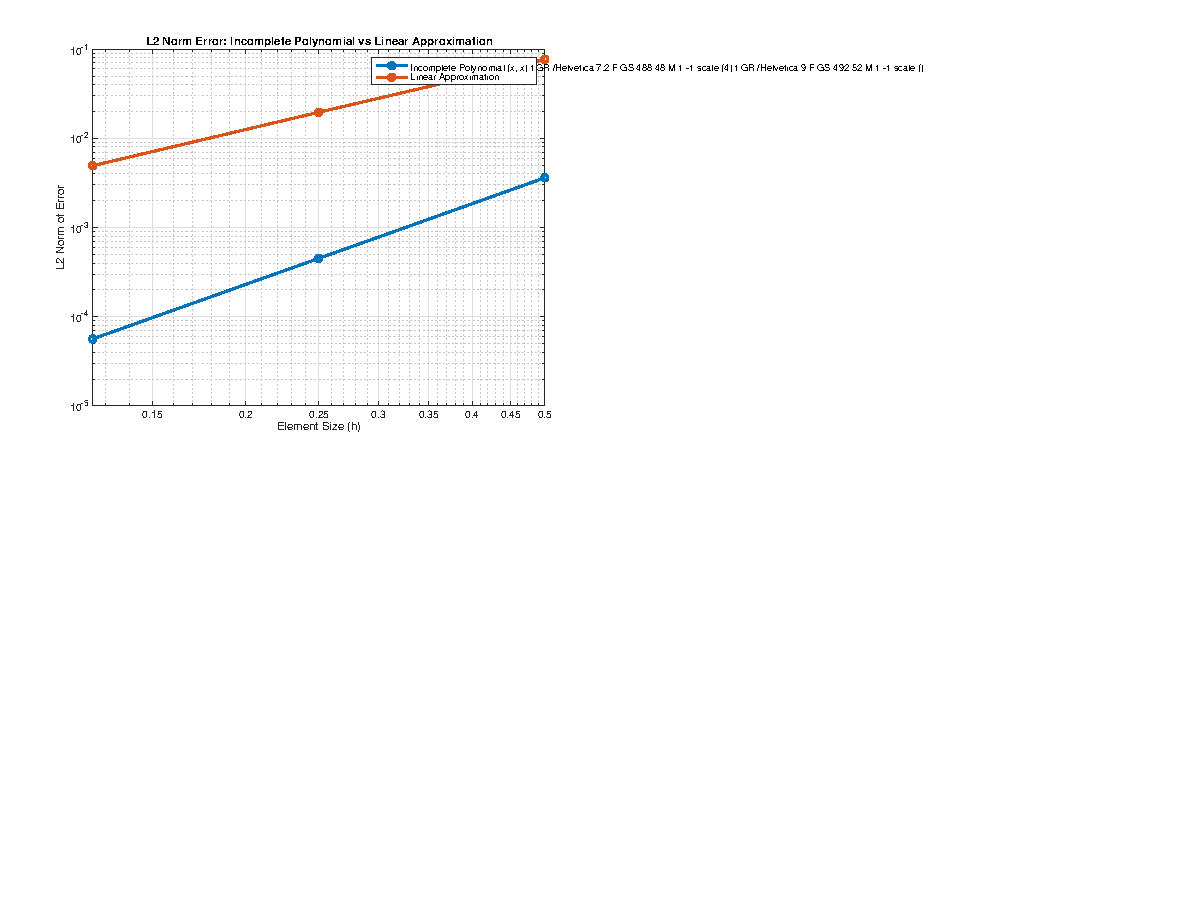
\includegraphics[width=\maxwidth{56.196688409433015em}]{figure_2.eps}
\end{center}
\begin{matlabcode}

% Optionally, compute and print the slopes of the log-log plots (rate of convergence)
p_incomplete = polyfit(log(element_sizes), log(error_L2_incomplete), 1);
p_linear = polyfit(log(element_sizes), log(error_L2_linear), 1);
fprintf('Slope of log-log plot (rate of convergence for incomplete polynomial): %.2f\n', p_incomplete(1));
\end{matlabcode}
\begin{matlaboutput}
Slope of log-log plot (rate of convergence for incomplete polynomial): 3.00
\end{matlaboutput}
\begin{matlabcode}
fprintf('Slope of log-log plot (rate of convergence for linear approximation): %.2f\n', p_linear(1));
\end{matlabcode}
\begin{matlaboutput}
Slope of log-log plot (rate of convergence for linear approximation): 1.98
\end{matlaboutput}

\begin{par}
\begin{flushleft}
Here is another attempt at trying to analyze the error of the element size. I think that this may be the best of the graphical representations.
\end{flushleft}
\end{par}

\end{document}
